\section{A felhasznált technológiák}
\subsection{Eclipse}

Az \textit{Eclipse} \cite{Eclipse} egy nyílt forráskódú, platformfüggetlen keretrendszer.
Első sorban fejlesztői környezetként használják a fejlesztők.
A keretrendszert tovább lehet bővíteni mindenféle \textit{plugin} telepítésével, így például modellezésre is alkalmas lehet.
A projektem során a következő \textit{Eclipse} \textit{plugin}-okat használtam::

\begin{itemize}
    \item \textit{Xtext} \cite{Xtext}
    \item \textit{Xtend} \cite{Xtend}
    \item \textit{Sirius} \cite{Sirius}
\end{itemize}

A munkafolyamat egy \textit{workspace}-en belül történik, ahol a fejlesztő létrehozhatja a saját projektjeit.
Több \textit{workspace}-t is létre lehet hozni és azok között váltani.

Különböző fajta projekteknek különböző nézetei lehetnek.
Például egy modellező projektnek van külön modell nézete az eszközön belül vagy egy \textit{Java} projektnek \textit{Java} nézete.
A nézetek az eszközön megjelenített szövegszerkesztő, fájlkezelő vagy egyéb funkció elhelyezéséért, megjelenítéséért felelnek.

\subsection{Xtext}

Az \textit{Xtext} \cite{Xtext} \textit{Eclipse} \textit{plugin}-nel programozási és \textit{domain} specifikus nyelveket lehet fejleszteni.
A nyelvünk elemeit és szabályait egy nyelvtan segítségével definiálhatjuk.
Az \textit{Xtext} keretrendszer több eszközt nyújt a nyelvünkhöz, például egy \textit{parser}-t, egy fordítót és egy szerkesztőt.
A \textit{plugin} még egy \textit{Xtend} alapú kódgenerátort is generál a nyelvünkhöz, amivel a nyelvünkhöz tetszőleges kódot tudunk generálni.

\begin{lstlisting}[language=java, frame=single, float=ht!, caption={Xtext nyelvtan elemei.},captionpos=b, label=XtextGrammar]
Scenario:
	'scenario' name=ID '{'
	scenariocontents+=ScenarioContent*
	'}'
;

ScenarioContent:
	alt+=Alt | message+=Message | par+=Par | loop+=Loop | paramConstraint+=ParameterConstraint

;

Message:
	LooseMessage | StrictMessage | PastMessage | FutureMessage | StrictFutureMessage
	| RequiredLooseMessage | RequiredStrictMessage | RequiredPastMessage | RequiredFutureMessage | RequiredStrictFutureMessage
	| FailMessage | FailStrictMessage | FailPastMessage
;

LooseMessage:
	'message' name=ID '(' (params+=Params | constantparams+=ConstantParams) ')'
	sender=[Object] '->' receiver=[Object]
	('clockConstraint' '{' cConstraint=ClockConstraintExpression '}')? 
	(resetclock=ResetClock)? ';'
;
\end{lstlisting}

A \ref{XtextGrammar}-es kódrészlet az \textit{Xtext} nyelvtan elemeit mutatja be.
Egy nyelvtani szabályt egy tetszőleges név megadásával hozhatunk létre, a szabályunkat pedig a név után lévő ":" és ";" közzé írhatjuk.
Idézőjelek közé írhatjuk a nyelvünkhöz tartozó kulcsszavakat, például \textit{'scenario'} vagy idézőjelek között kapcsos zárójel.
Ilyen kulcsszavak megadásával jól tudjuk formázni a nyelvtani szabályunkat.
Attribútumok megadásával tudjuk tárolni a nyelvi elemünk értékeit, változóit, például a \textit{name} attribútum egy \textit{ID} elemet tárol, ami egy azonosítónak felel meg.
Egy attribútumba több elemet is rakhatunk lista szerűen.
Ezt a \textit{*} karakterrel adhatjuk meg, például \textit{scenariocontents+=ScenarioContent*}, ahol a \textit{scenariocontents} több \textit{ScenarioContent}-beli elemet tárol.
A \textit{+=} karakterrel pakolhatjuk az új \textit{ScenarioContent}-jeinket a \textit{scenariocontents} tömbbe.

A nyelvtanukban megadhatunk elágazó szabályokat is a "|" karakterrel.
Ilyen szabály például a \textit{Message}.
Továbbá hivatkozhatunk már létrehozott nyelvi elemekre is a szabályunkban a "[]" szintakszissal.
Például a \textit{LooseMessage} \textit{sender} attribútuma egy már létrehozott \textit{Object} elemre hivatkozik.

A "?" karakter opcionális nyelvi elemek megadására szolgál.

Fordítás után a nyelvi elemeinkből \textit{Xtend} és \textit{Java} osztályok generálódnak.

\subsection{Xtend}

Az \textit{Xtend} \cite{Xtend} egy magasszintű programozási nyelv, amely a \textit{Java Virtual Machine} platformot használja.
Szintaktikailag és szemantikailag nagyon hasonlít a \textit{Java} nyelvhez, mondhatni a \textit{Java} kibővítése.
Az \textit{Xtend} fordító a létrehozott osztályokból \textit{Java} osztályokat generál.
Így akár könnyedén ki tudjuk szervezni a projektünket egy \textit{.jar} fájlba.

Egy nagyon hasznos funkciója az \textit{Xtend}-nek a \textit{template}, amely segítségével sablonokat hozhatunk létre a függvényeken belül, így megkönnyítve a kódgenerálást.
Így tudunk hivatkozni az \textit{Xtext} nyelvi elemeinkre függvény paramétereken keresztül és egyedi kódgenerátort fejleszteni a nyelvünkhöz.
A sablon függvényen belül a "«»" karaktereket használva tudunk hivatkozni az \textit{Xtext} nyelvi elemeinkre.

\begin{lstlisting}[language=java, frame=single, float=ht!, caption={Xtend template.},captionpos=b, label=XtendTemplate]
def compile(Scenario scenario)'''
	«FOR sc : scenario.scenariocontents»
		«FOR m : sc.message»
			«generateMessage(m)»
			a.collapse(b);
		«ENDFOR»
	«ENDFOR»
'''
\end{lstlisting}

A \ref{XtendTemplate} ábra egy \textit{Xtend} sablon függvényt mutat be.
Láthatjuk, hogy a "«»" karaktereket használva hivatkozhatunk a paraméterben átadott \textit{Xtext} nyelv béli objektum attribútumaira.
Itt például a \textit{Scenario} \textit{scenariocontents} tömbjén megyünk végig.

\subsection{Sirius}

A \textit{Sirius} \cite{Sirius} eszköz segítségével létrehozhatunk saját grafikus modellező alkalmazásainkat.
Egy szerkesztő környezetet alkothatunk, amivel a modellünk elemeit hozhatjuk létre, vagy szerkeszthetjük grafikusan.
A \textit{plugin} az \textit{Entity Modelling Framework} \cite{EMF} keretrendszert használja a modellek feldolgozásához és ilyen \textit{EMF} modelleket jelenít meg.
Ehhez az \textit{EMF} modellünk összes eleméhez meg kell adnunk egy megjelenítést.

Elkészíthetjük saját egyedi szerkesztőnket, de választhatunk a \textit{Sirius} által nyújtott szerkesztőkből is:
\begin{itemize}
	\item Diagram
	\item Szekvencia diagram
	\item Táblázat
\end{itemize}

Az egyes modell elemeinkhez tartozó grafikus megjelenítést egy \textit{viewpoint} létrehozásával tudjuk megtenni.
A \ref{sirius_viewpoint} ábrán látható egy példa \textit{viewpoint}.
A \textit{viewpoint}-hoz hozzá fűzhetünk egy \textit{representation}-t amely a konkrét megjelenítésünket tartalmazza.
Itt adhatjuk meg, hogy egyes modell elemeink milyen formában jelenjenek meg.

\begin{figure}[!ht]
    \centering
    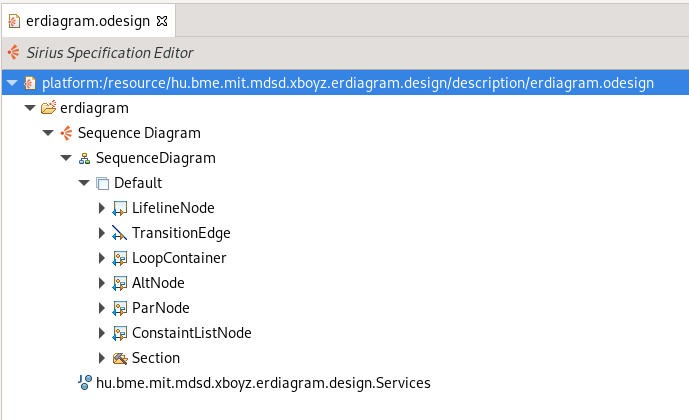
\includegraphics[width=150mm, keepaspectratio]{figures/sirius_viewpoint.png}
    \caption{\textit{Sirius} alkalmazáshoz tartozó \textit{viewpoint}.}
    \label{sirius_viewpoint}
\end{figure}

Emellett alkalmazhatunk feltételes megjelenítést is adott típusú modellelemünkre, ha az adott tulajdonságban eltér a többi elemtől.